\documentclass[paper=a4, fontsize=11pt,twoside]{article}

% -------------------------------------------------------------------- 
% General Page Layout
% --------------------------------------------------------------------
\usepackage[a4paper]{geometry} 
\usepackage[parfill]{parskip}
\setlength{\oddsidemargin}{5mm}  % Remove 'twosided' indentation
\setlength{\evensidemargin}{5mm}
%\usepackage{titlesec}
%\titleformat{\subsection}[runin]{\normalfont\bfseries}{\thesubsection.}{3pt}{}

% --------------------------------------------------------------------
% Encoding and Language Settings
% --------------------------------------------------------------------
\usepackage[T1]{fontenc} 
\usepackage[utf8]{inputenc}   
% encoding may need to be changed depending on the system
\usepackage[swedish]{babel} 
\usepackage{lipsum} % Lorem Ipsum

% --------------------------------------------------------------------
%  Utilities (colors, links, pictures, ect...)
% --------------------------------------------------------------------
\usepackage{xcolor}
\usepackage{hyperref}
\usepackage{graphicx}
\usepackage{amssymb}
\usepackage{epstopdf}
\usepackage[round]{natbib}
\usepackage{float}
\DeclareGraphicsRule{.tif}{png}{.png}{`convert #1 `dirname #1`/`basename #1 .tif`.png}

% -----------------------------------------------------------------------------%
% Title Page / Document Class Definitions (Please Don't Play With This)
% -----------------------------------------------------------------------------%

% Table of contents depth = section & subsection
\setcounter{tocdepth}{2}
																						
% Horizontal rule
\newcommand{\HRule}[1]{\rule{\linewidth}{#1}}   															
																									
% Document Number
\newcommand{\documentNumber}[1]{\centering PUSP1742#1 \\[1.0cm]}	 										
																									
% Document Version
\newcommand{\documentVersion}[1]{\centering \small{v.#1} \\[1.0cm]}

% Group Responsible
\newcommand{\documentResponsible}[1]{\centering  Ansvarig Grupp: #1}

% Document Creator Group
\newcommand{\documentCreator}[1]{\centering Uppgjord Av: #1}	 									
																								
% Title
\makeatletter \def\printtitle{ {\centering \@title\par}} \makeatother
																									
% Author .. not really used, but it can stay in case
\makeatletter \def\printauthor{ {\centering \large \@author}} \makeatother
																									
\newcommand{\grouptitlepage}[4]{ 
\title{
\documentNumber{#1}																						
\documentVersion{#2}																				
\HRule{0.5pt} \\ % Upper rule 
\LARGE \textbf{\uppercase{#3}} \\
\large \textbf{\uppercase{ETSF20 Grupp 2}} 
\HRule{2pt} \\ [1.5cm]    
\normalsize            
\documentResponsible{#4} \\ 
\documentCreator{#4}  
}																							
\maketitle																							
\thispagestyle{empty} 																	\newpage 				
 
}
% \grouptitlepage{doc number}{Version Number}{doc title}{group responsible for
% doc}
% --------------------------------------------------------------------------------%
% Title Page / Document Class Definitions (Please Don't Play With This)
% --------------------------------------------------------------------------------%


% \date{}                                            
% Activate to display a given date or keep commented for current date


% -------------------------------------------------------
% DOCUMENT START (YOU CAN IGNORE EVERYTHING ABOVE HERE)
% -------------------------------------------------------
\begin{document}

% ---------------------------------------------------------------------------------------------------------------------------------------
% Title Page START: \grouptitlepage{doc number}{Version Number}{doc title}{group responsible for doc}		
%---------------------------------------------------------------------------------------------------------------------------------------
\grouptitlepage
%Document Code Number (same as time reports)
{12}
%Document Version Number										
{1.0}
%Document Title		Dokumentmall							
{SRS - Kravspecifikation}
%Group Responsible For Document									
{(SG) Systemgrupp}	
% -------------------------------------------------------------------------------------------------------------
% Title Page END				
% -------------------------------------------------------------------------------------------------------------
\tableofcontents
\section{Introduktion}
Detta dokument beskriver kraven för ett tidrapporteringssystem, baserat på “BaseBlockSystem”. Det är ett system där man främst kan skapa och lagra tidrapporter för enskilda medlemmar i ett projekt. Se referens dokumentet nedan för mer ingående förklaring av systemet.
\section{Referensdokument}
Base Block System SRS: \textbf{\textit{PUSS12002 version: 1.0}}  gäller för alla punkter	 om det inte är specificerat i respektive underrubrik att det som står i \textbf{\textit{PUSS12002 version: 1.0}}  utgår för specifik del.

\newpage
\section{Bakgrund och Mål}
\subsection{Huvudmål:}
De huvudsakliga målet med systemet är att erbjuda ett funktionellt tidrapporteringssystem som bygger vidare på ett redan givet “BaseBlockSystem”. Detta ska kunna användas av projektgrupper för att enkelt kunna rapportera in arbetstid.
\subsection{Aktörer och deras mål:}
Följande huvudaktörer använder systemet:
\subsubsection{Användare:}
En användare ska ha en roll i projektgruppen. Den ska kunna tidsrapportera, ändra en osignerad tidsrapport. Användaren ska kunna se en sammanställning av sin totala rapporterade tid. Det huvudsakliga målet för en användare är att på ett simpelt sätt kunna tidsrapportera.
\subsubsection{Projektledare:}
En projektledare är en specifik användare som har tilldelats rollen “Projektledare” av administratören. En projektledare ska, utöver det en användare kan göra, kunna tilldela de olika rollerna till användarna. Projektledare ska kunna signera och annullera rapporter från övriga projektmedlemmar. Projektledaren ska kunna se en sammanställning av all den totala tid som rapporterats i projektet. De huvudsakliga målen för en projektledare är att kunna rapportera tid, signera tidsrapporter och tilldela roller till projektmedlemmarna. 
\subsubsection{Administratör:}
En administratör ska kunna lägga till och ta bort användare i systemet. Den ska även kunna tilldela rollen “Projektledare” till användare. Administratören ska kunna skapa och ta bort projektgrupper och kunna tilldela användare till dessa projektgrupper. Det huvudsakliga målen för en administratör är att kunna lägga till och ta bort användare, lägga till och ta bort projektgrupper och kunna tilldela rollen “Projektledare”.



%4
\section{Terminologi}
\paragraph{Tidrapport}
\flushleft
Dokument som används för att rapportera de timmar man lagt på olika områden i ett arbete/projekt. Används i samband med löne-och projektredovisning.
\paragraph{Administratör}
\flushleft
Någon som förvaltar en organisation. I detta projektets fall, ett system.
\paragraph{Förvaltning}
\flushleft
Vara ansvarig för ett visst arbete till någons räkning, eller ha hand om en verksamhet.
\paragraph{Annullera}
\flushleft
Upphäva, ogiltigförklara något, t.ex annullera en signering av en tidsrapport.
\paragraph{Projekt}
\flushleft
Ett uppdrag som utförs av en viss arbetsorganisation för att åstadkomma ett visst resultat. 
\paragraph{Signering}
\flushleft
Bekräftar en tidrapport och sätter den i ett stadie där den inte kan ändras om inte projektledare häver signeringen.

%5
\section{Kontextdiagram}
\begin{figure}[H]
\centering
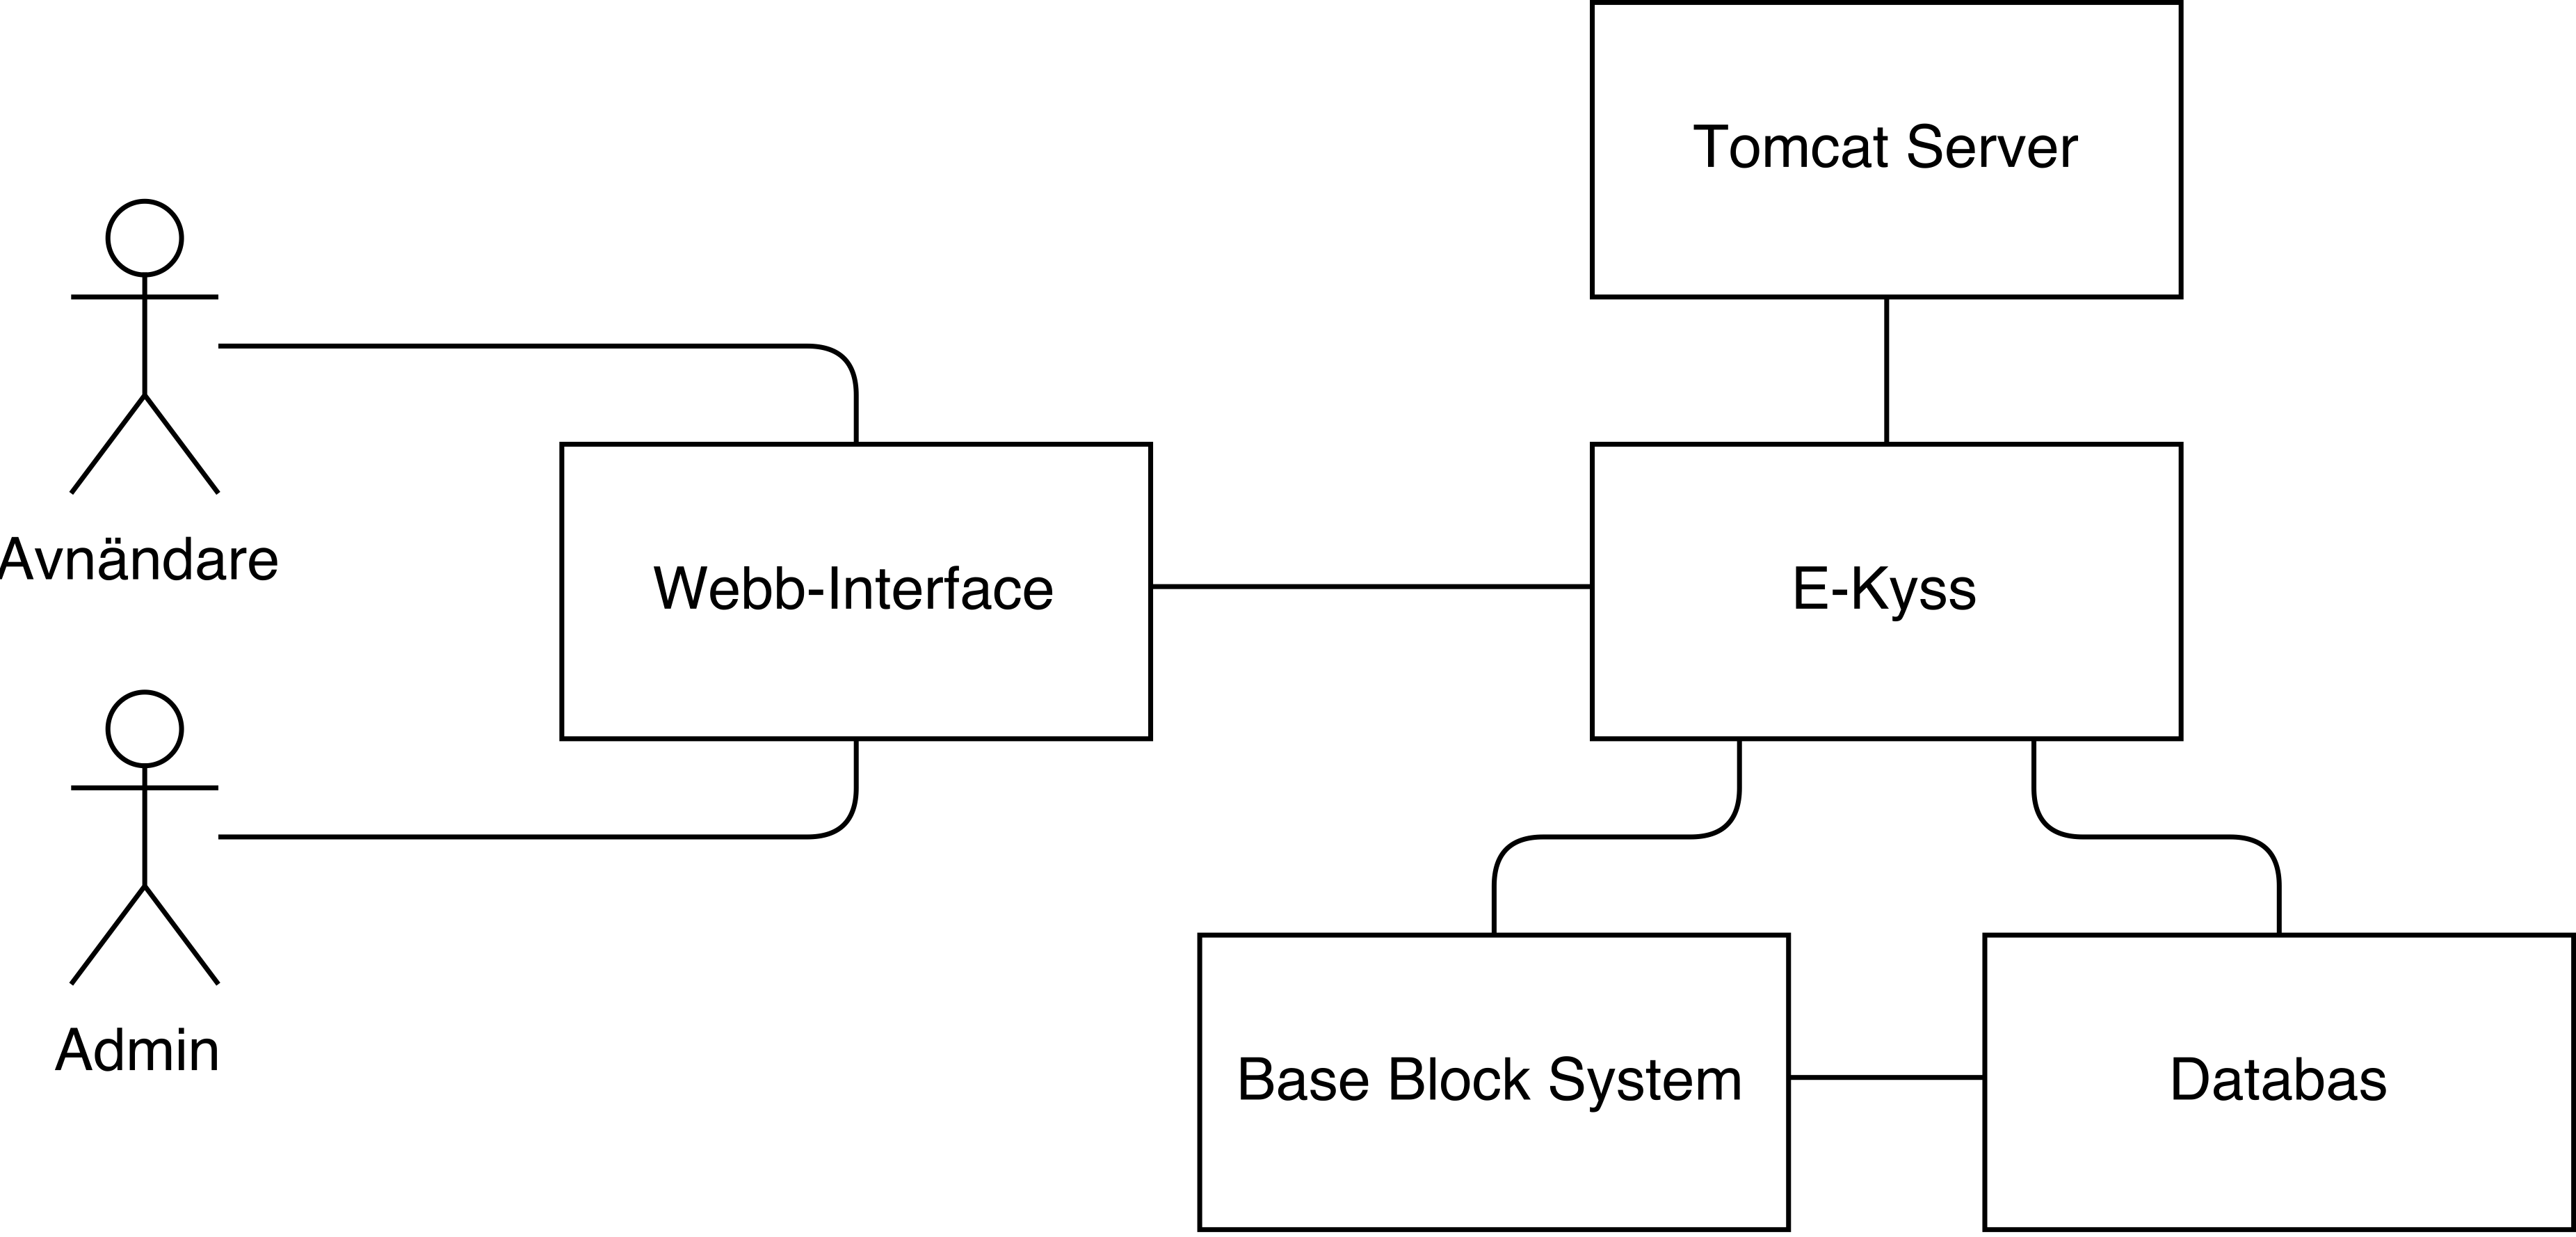
\includegraphics[width = 12cm]{Kontext_Diagram.png} 
\caption{Kontextdiagram}
\end{figure}

%6
\section{Projektkrav}
\subsection{Huvudkrav:}
\subsubsection{Krav:}
Systemet skall vara en vidareutveckling av grundsystemet ''Base Block System''

%7
\section{Kvalitetskrav}
\subsection{Prestanda:}
\subsubsection{Krav:}
När systemet används på en dator i någon sal på LTH Campus Helsingborg i C-Byggnaden ska svarstiden på godtycklig förfrågan ges inom 1.0 sekunder för 95\% av fallen


% TODO Bilder nedan för designkrav


%8
\section{Designkrav}
\subsection{Interface:}
\subsubsection{Krav:} Krav på design på inloggnings-sidan kan ses i figur 2.
\begin{figure}[H]
\centering
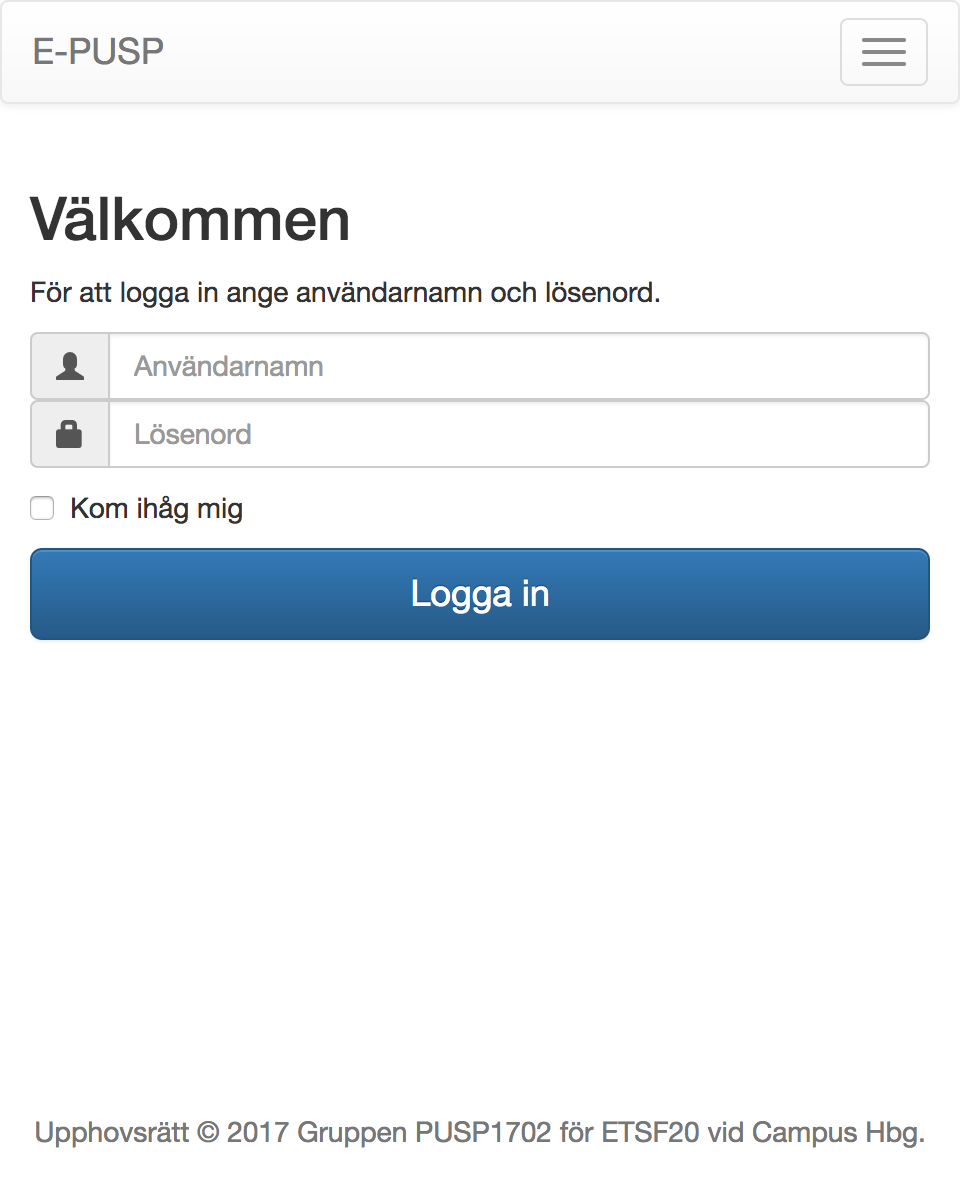
\includegraphics[width=8cm]{login}
\caption{Inloggnings-sidan}
\end{figure}

\newpage
\subsubsection{Krav:} Krav på design av tidsrapporteringen kan ses i figur 3.
\begin{figure}[H]
\centering
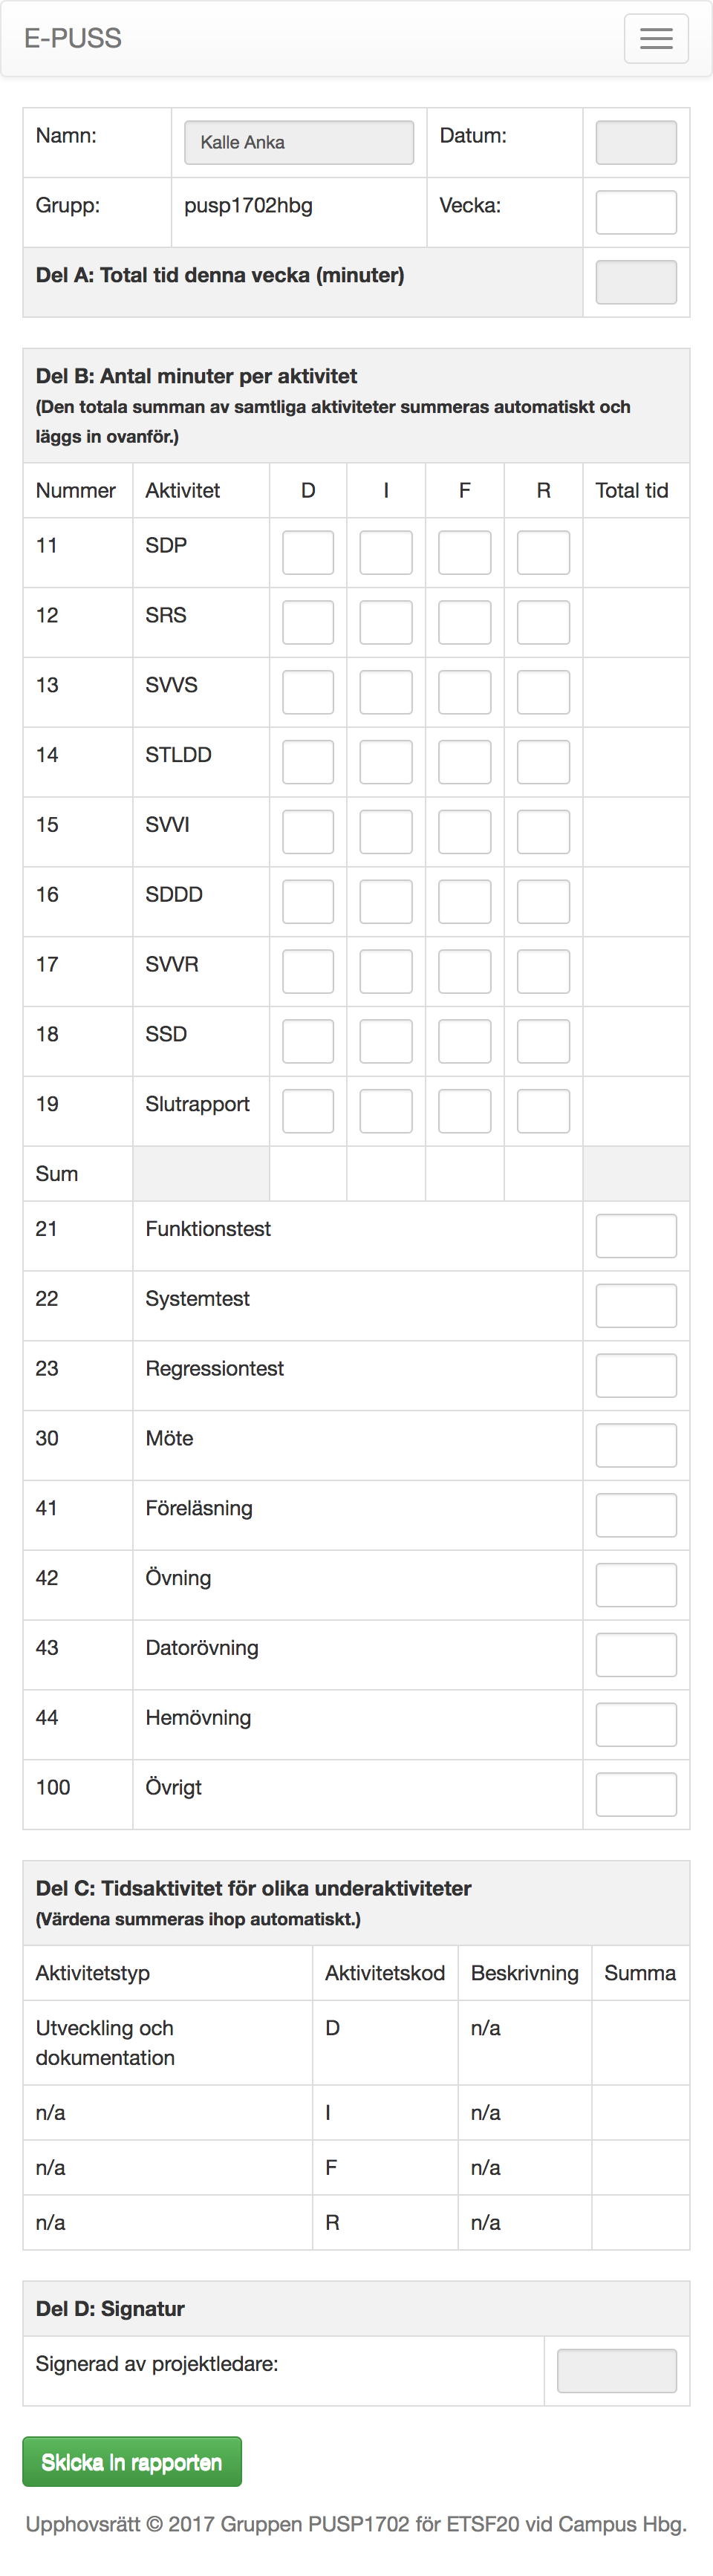
\includegraphics[width=5cm]{prtscn-tidrapportering.png}
\caption{tidsrapporteringen}
\end{figure}


%9
\section{Funktionella Krav}
\subsubsection{Allmänna krav:}
Kraven om funktionalltet i grundsystemet skall även gälla för detta system.
\subsubsection{Allmänna krav:}
En loggfil skapas för varje projektgrupp när projektgruppen skapas.
\subsubsection{Allmänna krav:}
Varje ändring av projektgruppens data sparas i sin loggfil.
\subsubsection{Allmänna krav:}
När en grupp tas bort sin logfil också raderas.
\subsubsection{Allmänna krav:}
En ändring i logfilen ska innehålla en tidsstämpel följt av användaren som gjorde ändringen.

\subsection{Administratör:}

\subsubsection{Krav:} Följande scenario ska stödjas av systemet.
\paragraph{Scenario:}
Admin vill lägga till en projektgrupp i systemet.
\paragraph{Förkrav:}
Admin är inloggad.
\begin{enumerate}
\item Admin går till sidan för hantering av projektgrupper
\item Admin väljer att lägga till projektgrupp
\item Admin uppmanas att mata in namn på projektgrupp
\item Projektgrupp skapas
\item Admin ser en uppdatering av sidan
\end{enumerate}

\subsubsection{Krav:} 
Följande scenario ska stödjas av systemet.
\paragraph{Scenario:}
Admin vill ta bort minst en projektgrupp i systemet.
\paragraph{Förkrav:}
Admin är inloggad. Det finns minst en projektgrupp.
\begin{enumerate}
\item Admin går till sidan för hantering av projektgrupper
\item Admin väljer vilken/vilka projektgrupper som ska tas bort genom markering i kryssrutor
\item Admin trycker på en knapp för att radera valda projektgrupper
\item Admin ser en varningsruta som bekräftar att projektgrupper ska raderas
\item Projektgruppen/grupperna som valts raderas
\item Admin ser en uppdatering av sidan
\end{enumerate}

\subsubsection{Krav:} Följande scenario ska stödjas av systemet. 
\paragraph{Scenario:}
Admin skall utse projektledare i system utan användare.
\paragraph{Förkrav:}
Admin är inloggad. Ingen användare finns i systemet. Det finns minst en projektgrupp i systemet.
\begin{enumerate}
\item Admin går till sida för att hantera medlemmar
\item Admin lägger till användare i en projektgrupp
\item Admin tilldelar användaren rollen projektledare
\item Admin ser en uppdatering av sidan
\end{enumerate}

\subsubsection{Krav:} Följande scenario ska stödjas av systemet. 
\paragraph{Scenario:}
Admin skall utse projektledare i system med användare.
\paragraph{Förkrav:}
Admin är inloggad. Det finns minst en användare i systemet. Det finns minst en projektgrupp i systemet.
\begin{enumerate}
\item Admin går till sidan för hantering av användare
\item Admin utser en användare och tilldelar denna rollen projektledare
\item Användaren har enbart rollen projektledare
\item Admin ser en uppdatering av sidan
\end{enumerate}

\subsubsection{Krav:} Följande scenario ska stödjas av systemet. 
\paragraph{Scenario:}
Admin vill lägga till en användare i systemet.
\paragraph{Förkrav:}
Admin är inloggad. 
\begin{enumerate}
\item Admin går till sidan för hantering av användare
\item Admin väljer att lägga till en användare
\item Admin uppmanas att mata in namn på den nya användaren
\item Admin uppmanas att mata in e-post som kopplas till den nya användaren
\item Användaren skapas med valt användarnamn och e-post
\item Användaren får e-post med användarnamn och slumpat lösenord
\item Admin ser en uppdatering av sidan
\end{enumerate}

\subsubsection{Krav:} Admin ska kunna ta bort flera medlemmar samtidigt genom att kryssa i en ruta för vardera medlem som ska raderas. Sedan ska admin trycka på en knapp för att ta bort dessa.

\subsubsection{Krav:} Admin ska inte kunna ta bort sig själv.

\subsubsection{Krav:} Följande scenario ska stödjas av systemet. 
\paragraph{Scenario:}
Admin vill ta bort användare i systemet.
\paragraph{Förkrav:}
Admin är inloggad. Det finns minst en användare i systemet.
\begin{enumerate}
\item Admin går till sidan för hantering av användare
\item admin markerar vilken/vilka användare som ska raderas
\item Användarna raderas ur systemet
\item Admin ser en uppdatering av sidan
\end{enumerate}

%------------------------------------------------------------------------------------------------------------
%Projektledare start
%------------------------------------------------------------------------------------------------------------

\subsection{Projektledare:}

\subsubsection{Krav:} En projektledare ska kunna tilldela roller till projektmedlemmarna i projektgruppen.

\subsubsection{Krav:}
Följande scenario ska stödjas av systemet.
\paragraph{Scenario:}
Projektledare tilldelar roll till projektmedlem.
\paragraph{Förkrav:}
Användare är projektledare i gruppen. Minst en användare finns i systemet.
\begin{enumerate} 
\item Projektledare klickar på ”Main”
\item Projektledare klickar vidare på ”Organize group”
\item En ny sida visas med en lista på medlemmar i projektgruppen.
\item Projektledare klickar på roll-alternativ på medlem
\item Projektledare ändrar/tilldelar rollen
\item Tryck på knappen ”Update group”
\item Projektledare ser en uppdatering av sidan som visas i steg 3
\end{enumerate}

\subsubsection{Krav:}
Projektledaren ska kunna ändra projektmedlemmarnas roller i projektgruppen.

\subsubsection{Krav:}
De roller som ska finnas tillgängliga är:
\begin{enumerate}
\item[]
\begin{enumerate}
\item Projektgrupp
\item Systemgrupp
\item Utvecklingsgrupp
\item Testgrupp
\end{enumerate}
\end{enumerate}

\subsubsection{Krav:}
Projektledaren ska kunna signera och godkänna tidrapporter för varje medlem i gruppen.

\subsubsection{Krav:}
Följande scenario ska stödjas av systemet.
\paragraph{Scenario:}
Projektledare ska signera veckorapporter.
\paragraph{Förkrav:}
Användare är projektledare i gruppen.
\begin{enumerate}
\item Projektledaren klickar på ”Time Reporting”
\item Projektledaren klickar på ”Sign Time Reports”
\item En lista kommer upp med alla veckorapporter
\item Projektledaren markerar rapporterna som ska signeras och klickar på knappen ”Sign”
\item När Projektledaren signerat rapporterna, uppdateras sidan och visar en uppdaterad lista av alla veckorapporter
\end{enumerate}

\subsubsection{Krav:}
Signeringen av tidrapport sker veckovis.

\subsubsection{Krav:}
Projektledarens egna tidrapport signeras direkt vid tryckning av submit-knappen.

\subsubsection{Krav:}
Följande scenario ska stödjas av systemet.
\paragraph{Scenario:} Annullering av redan signerad tidrapport.
\paragraph{Förkrav:} Projektledaren är inloggad.
\begin{enumerate}
\item Projektledare klickar på ”Time reporting”
\item Projektledare klickar på ”Unsign reports”
\item Projektledaren kryssar för dom signerade rapporter som ska annulleras
\item Projektledaren klickar sedan på ”Submit changes”
\end{enumerate}

\subsubsection{Krav:}
Projektledaren ska, i menyn, ha följande länkar:
\begin{enumerate}
\item[]
\begin{enumerate}
\item ”Organize Group”
\item ”Sign reports”
\item ”Unsign reports”
\item ”View all reports”
\end{enumerate}
\end{enumerate}

\subsubsection{Krav:}
Projektledare ska kunna generera sammanställning över all tid som rapporterats i projektet.


\subsubsection{Krav:}
Projektledaren ska kunna se statistik för tidsrapporter i projektet för varje medlem.
Tidsrapporter ska kunna summeras och kunna visa tidsåtgång per:
\begin{enumerate}
\item[]
\begin{enumerate}
\item Användare
\item Roll
\item Aktivitet
\item Vecka
\item Fas
\item Dokument
	\end{enumerate}
\end{enumerate}
\subsubsection{Krav:}
Projektledaren ska i statistiken kunna se start för varje fas.
\subsubsection{Krav:}
Projektledaren ska i statistiken kunna se slut för varje fas.

%---------------------------------------------------------------------------------------------------------
%Projektledare slut (that's not a very nice thing to call me...)
%---------------------------------------------------------------------------------------------------------

\subsection{Användare:}
\subsubsection{Krav:} En användare ska kunna tidrapportera till det projekt den är medlem i.

\subsubsection{Krav:} Följande scenario ska stödjas av systemet.
\paragraph{Scenario:} Användare vill skriva en tidrapport.
\paragraph{Förkrav:}
Användare är inloggad i systemet.
\begin{enumerate}
\item Användaren går till sidan för hantering av tidrapport
\item Användaren får se en sammanställning med all tidigare rapporterad tid
\item Användaren trycker på en knapp för att skapa ny tidrapport
\item Användaren fyller i fält med dem aktuella tiderna för de olika aktiviteterna, fält kan lämnas tomma om ingen tid har lagts på aktiviteten
\item	Användaren trycker på en knapp för att skicka tidrapporten
\item Tidrapporten skickas till projektledaren för signering
\item Användaren ser en uppdatering av sidan
\end{enumerate}

\subsubsection{Krav:} En användare som är medlem i ett projekt ska kunna uppdatera osignerade tidrapporter i det projektet.

\subsubsection{Krav:} En användare som är medlem i ett projekt ska kunna ta bort sina egna osignerade tidrapporter i det projektet.

\subsubsection{Krav:}En användare ska kunna se all sin tidigare rapporterad tid.

\subsubsection{Krav:}En användare får endast ha ingen eller en roll i projektgruppen.

\subsubsection{Krav:} Följande scenario ska stödjas av systemet.
\paragraph{Scenario:}Användare vill uppdatera i tidrapport.
\paragraph{Förkrav:}
Användare är inloggad i systemet, tidsrapport är osignerad.
\begin{enumerate}
\item Användaren klickar på ”Time Reporting”
\item	Användaren klickar på ”Edit time report”
\item	Användaren kommer till en sida som innehåller en meny med användarens osignerade tidrapporter
\item Användaren klickar på en tidrapport
\item	En sida öppnas som visar aktuell tidrapport i form av en tabell med de gamla värdena ifyllda
\item	Användaren ändrar/lägger till värden i tidrapporten
\item	Användaren klickar på “Submit Change”
\item Användaren ser en uppdaterad sida med bekräftelsertuta att ändring utförts
\item	Den gamla tidrapporten försvinner och den ändrade tidrapporten skickas vidare för signering
\item	”Time Reporting” sidan visas
\end{enumerate}

\newpage
\subsubsection{Krav:}Följande scenario ska stödjas av systemet.
\paragraph{Scenario:}Användare vill se en sammanfattning av sin rapporterade tid.
\paragraph{Förkrav:}
Användaren är inloggad i systemet.
\begin{enumerate}
\item  Användaren klickar på ”Time Reporting” i menyn
\item  En ny sida visas som innehåller alternativ för tidrapportering samt en sammanställning för den totalt rapporterade tiden för användaren i form av en tabell
\end{enumerate}

\subsubsection{Krav:} Följande scenario ska stödjas av systemet.
\paragraph{Scenario:}Användare vill ändra lösenord.
\paragraph{Förkrav:}
Användare är inloggad i systemet.
\begin{enumerate}
\item	Användaren trycker på ”Change Password” i menyn
\item	En sida visas som innehåller relevanta textboxar
\item	Användaren fyller i nuvarande lösenord i första textboxen
\item	Användaren fyller i det nya lösenordet i den andra textboxen
\item	Användaren upprepar det nya lösenordet i den tredje textboxen
\item	Användaren trycker på knappen “Change Password”
\item	Lösenordet för användaren ändras i systemet. Detta visas på följande sida
\end{enumerate}

\subsubsection{Krav:}Följande scenario ska stödjas av systemet.
\paragraph{Scenario:}Användare vill ändra lösenord (ogiltig inmatning).
\paragraph{Förkrav:}
Användaren är inloggad i systemet.
\begin{enumerate}
\item  Användaren trycker på “Change Password” i menyn
\item	 En sida visas som innehåller relevanta textboxar
\item	Användaren fyller i nuvarande lösenord i första textboxen
\item	Användaren fyller i det nya lösenordet som inte uppfyller krav 6.2.3 i PUSS12002 version: 1.0 för “BaseBlockSystem” i den andra textboxen
\item	Användaren upprepar det nya lösenordet i den tredje textboxen
\item	Användaren trycker på knappen “Change Password”
\item	Lösenordet ändras inte och ett felmeddelande visas
\item Användaren skickas tillbaka till steg 2
\end{enumerate}


\end{document}
